\setcounter{section}{3}
\setcounter{subsection}{3}
\setcounter{subsubsection}{1}
\subsubsection{The rate monotonic schedule.}

\begin{enumerate}[label=\textbf{\arabic*})]
\item \textbf{Calculating utilization}

The utilization of a periodic task $\tau_i(T_i,C_i)$ is defined as:
\[u_i = \frac{C_i}{T_i}\]
The total utilization for a set of tasks is defined as:
\[U = \sum_{i=1}^{n} u_i\]

The 3 tasks given are:
\[\tau_i(\phi_i, T_i, C_i, D_i)\]

\[\tau_1(100, 300, 100, 300)\]
\[\tau_2(100, 400, 100, 400)\]
\[\tau_3(100, 600, 100, 600)\]

Their respective utilizations are:
\[u_1 = \frac{C_1}{D_1} = \frac{100}{300} = \frac{1}{3}\]
\[u_2 = \frac{C_2}{D_2} = \frac{100}{400} = \frac{1}{4}\]
\[u_3 = \frac{C_3}{D_3} = \frac{100}{600} = \frac{1}{6}\]

The total utilization $U$ can thus be calculated:
\[U = \frac{1}{3} + \frac{1}{4} + \frac{1}{6} = \frac{9}{12} = \frac{3}{4} = 0.75\]

The hyperperiod $H$ is defined as the least common multiplier from the set of task periods:
\[H = lcm(T_1, T_2, T_3) = lcm (300, 400, 600) = 1200\]

According to RMS the priorities should therefore be:
\[P_1 > P_2 > P_3\]

For one hyperperiod of 1200ms the schedule should look like this:

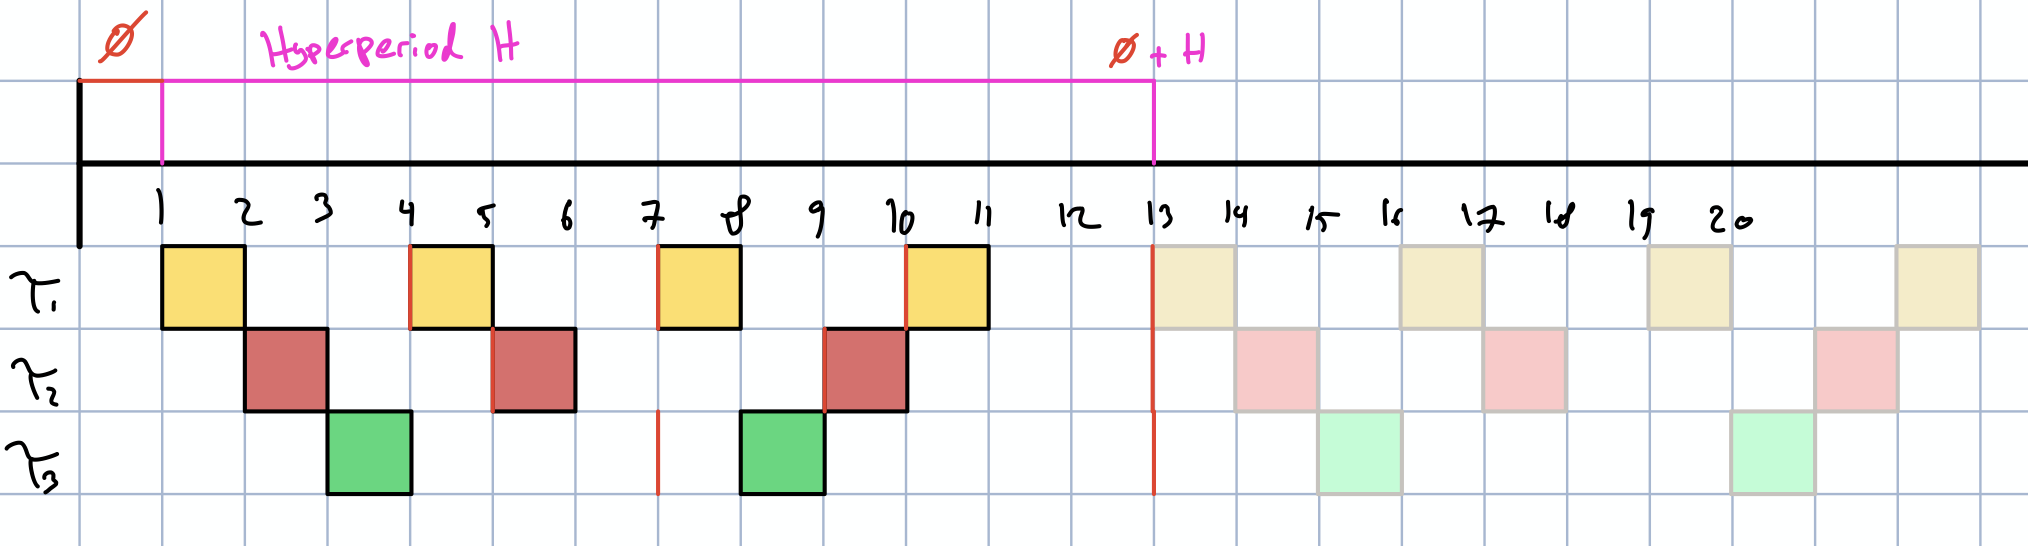
\includegraphics[width=0.9\linewidth]{1-rate-monotonic-schedule}

\item \textbf{Calibrating execution time}

Constraining the execution of the program to use only a single CPU core using taskset was made possible on a macOS system by using a virtual machine. The calibration parameter was set to \textbf{1208} which produced the following output:
\begin{figure}[H]
    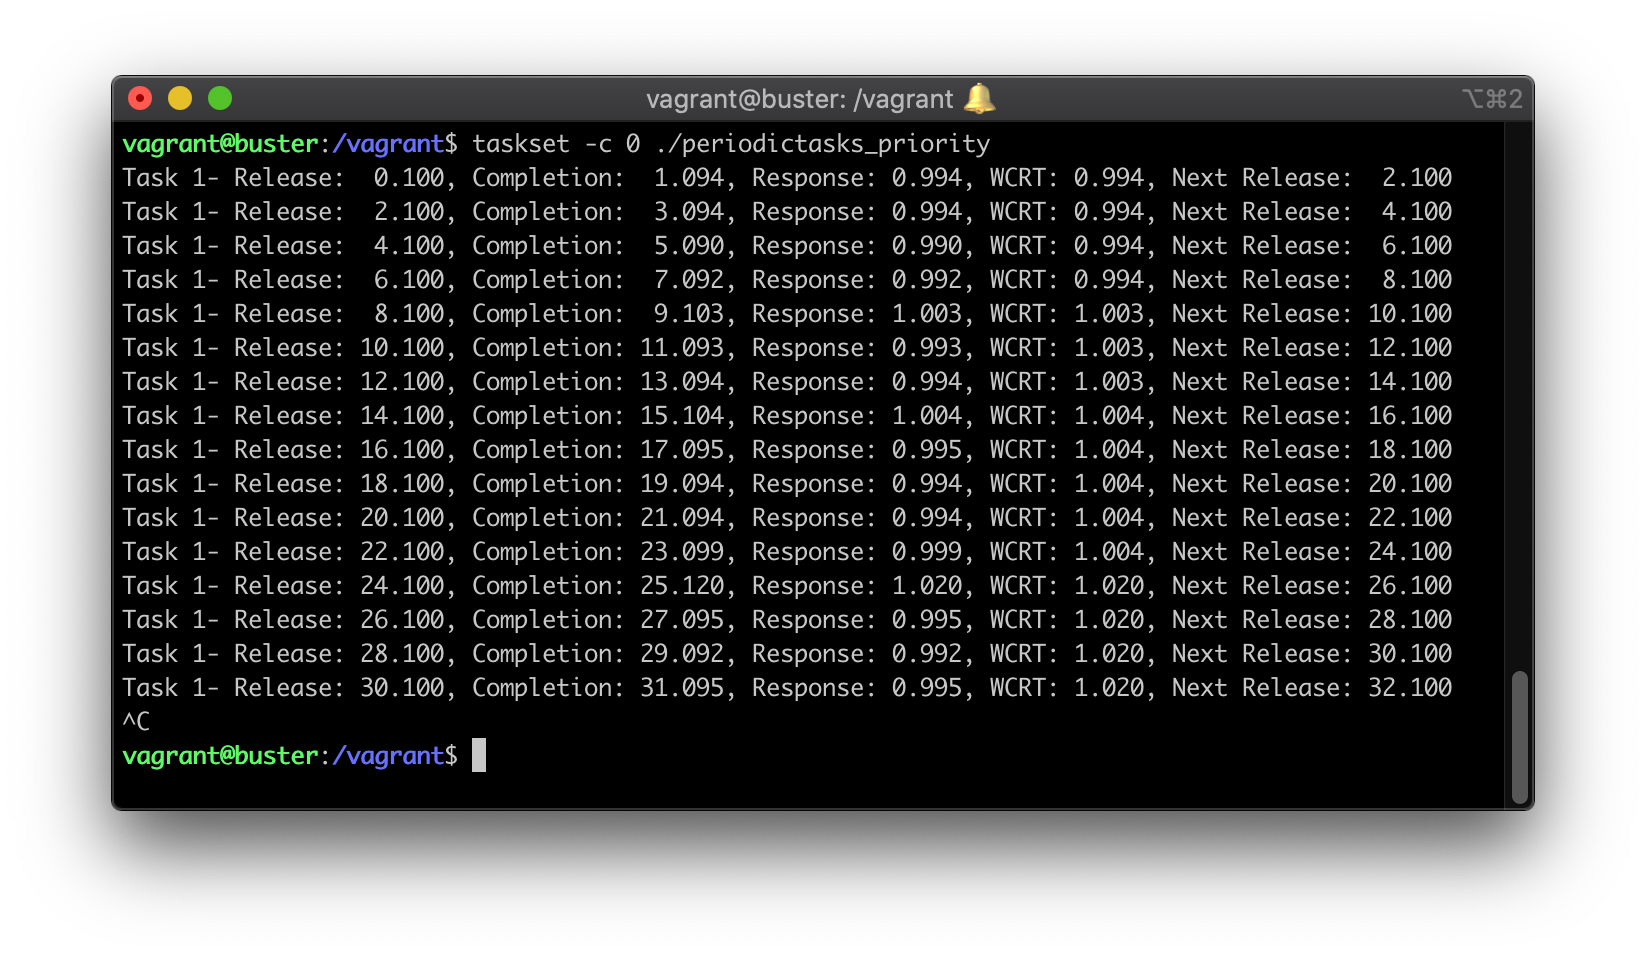
\includegraphics[width=\linewidth]{2-periodictasks-priority-output}
\end{figure}
\item \textbf{Implementing the periodic task set $\Gamma_1$}

Running the rms on a single core produces the following output:
\begin{figure}[H]
    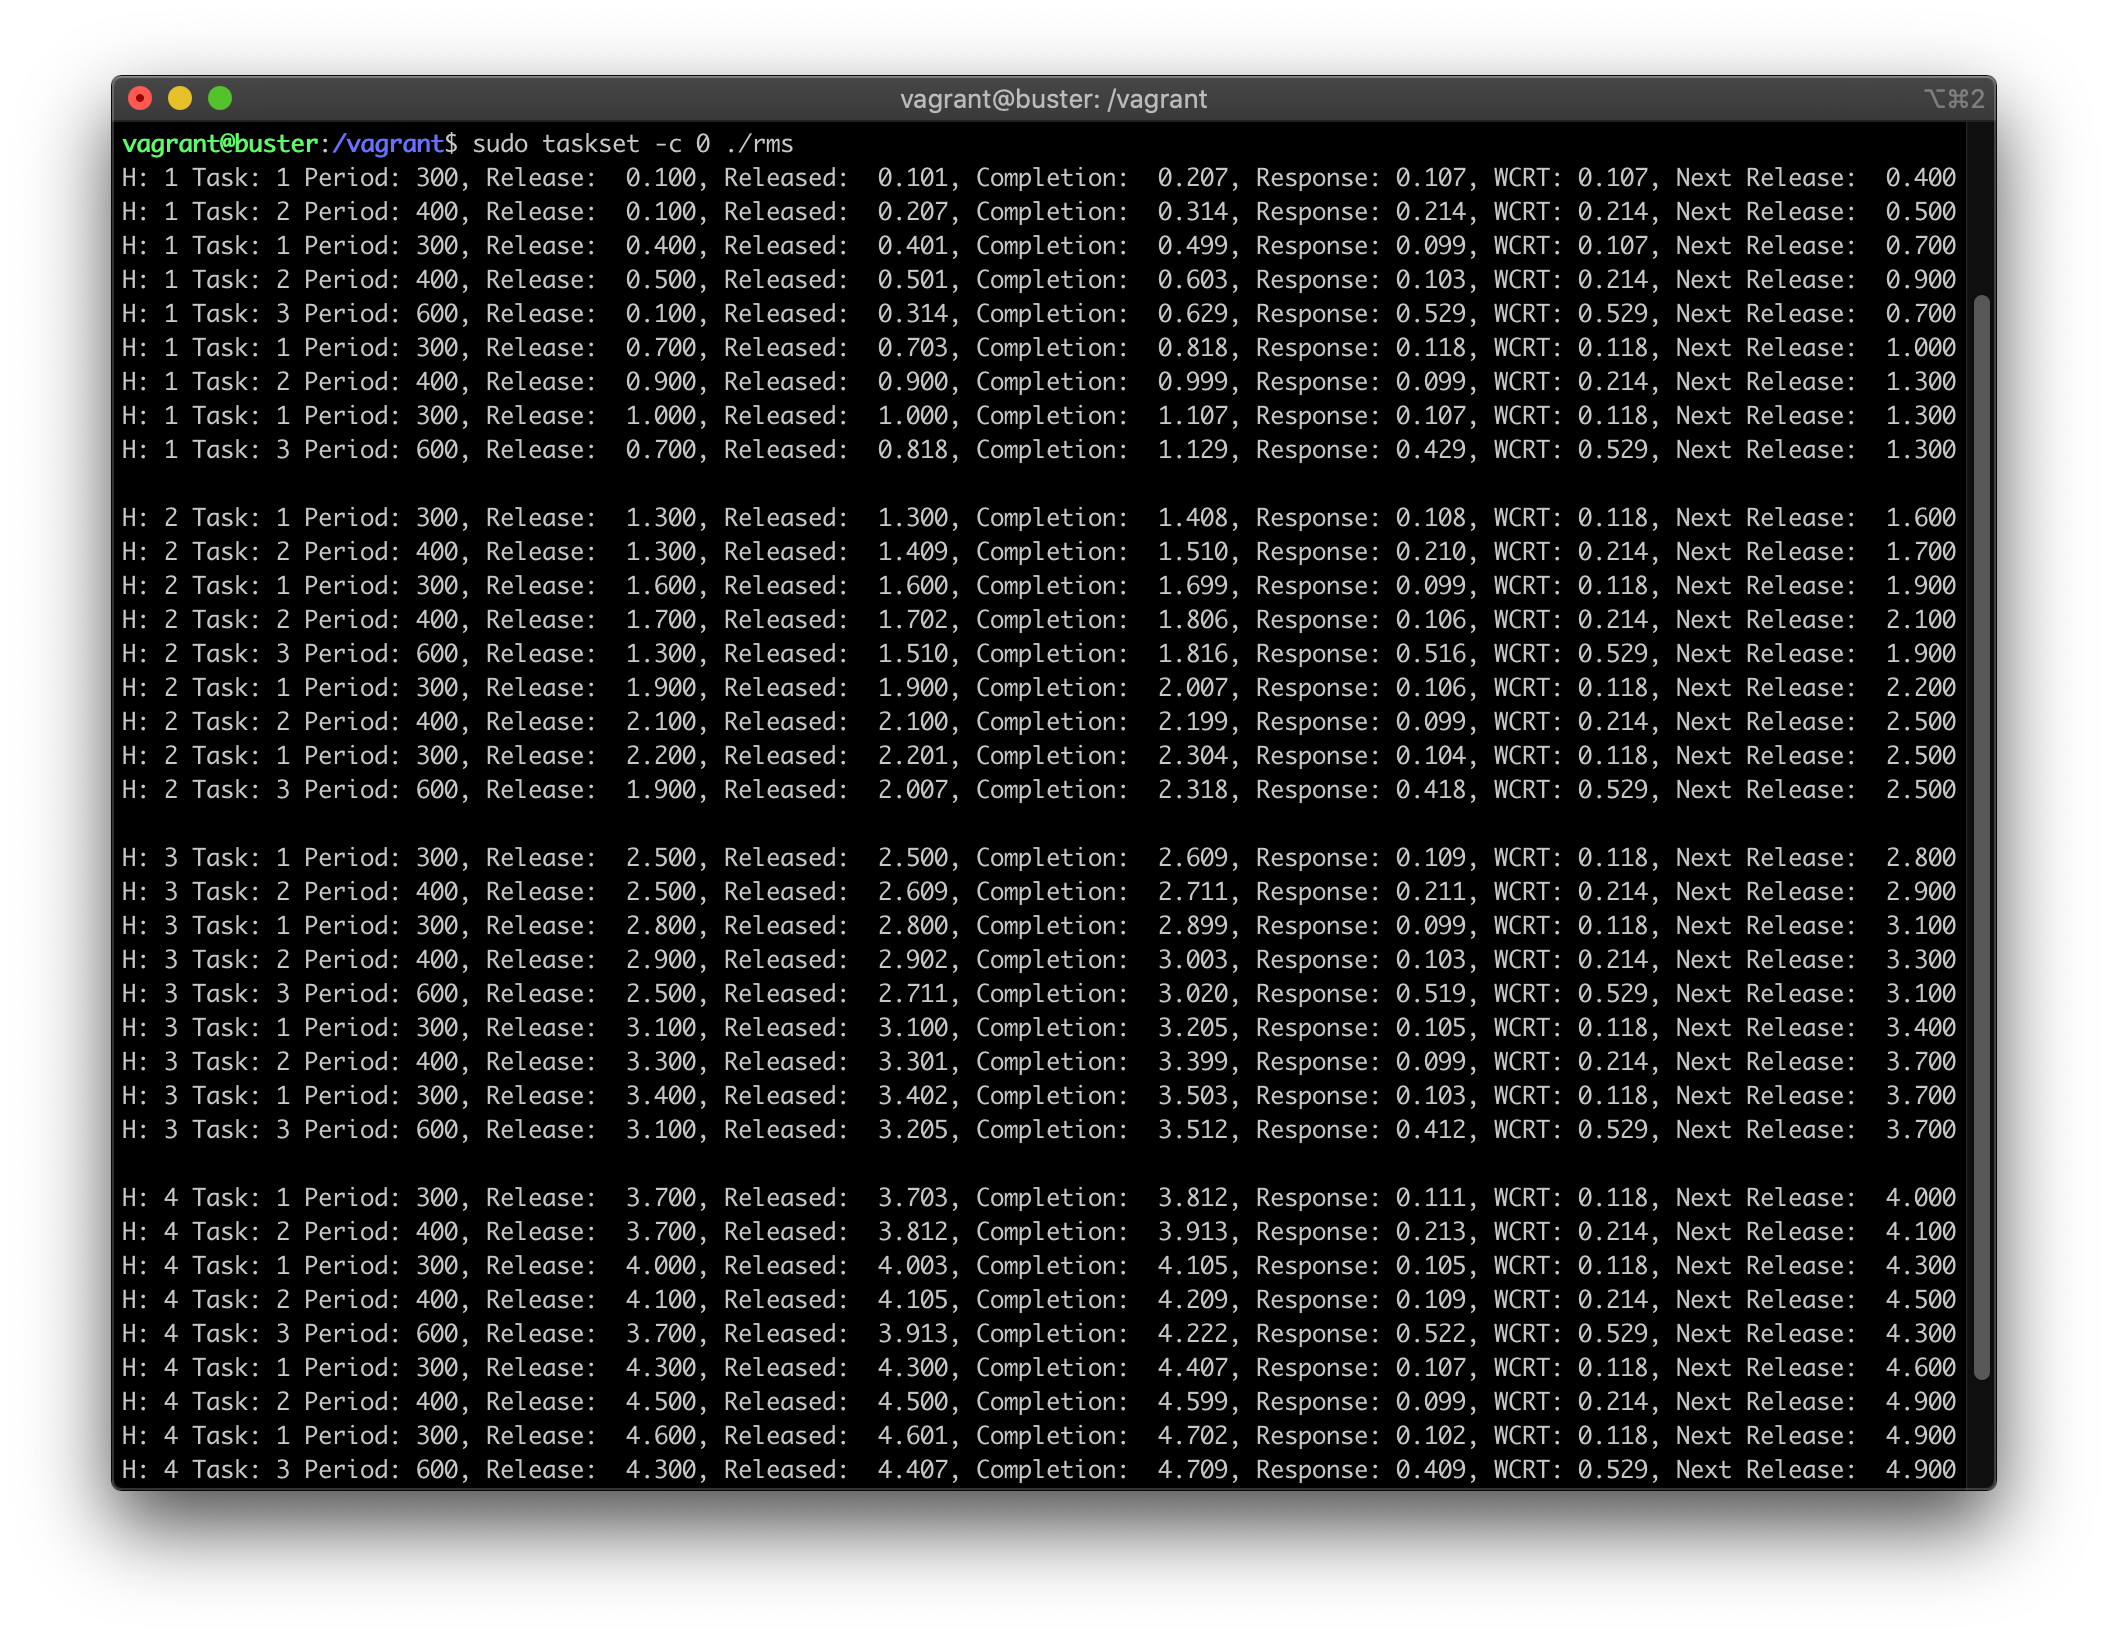
\includegraphics[width=\linewidth]{3-rms-output}
\end{figure}

\item \textbf{Adding the additional task  $\tau_4$}

\begin{figure}[H]
        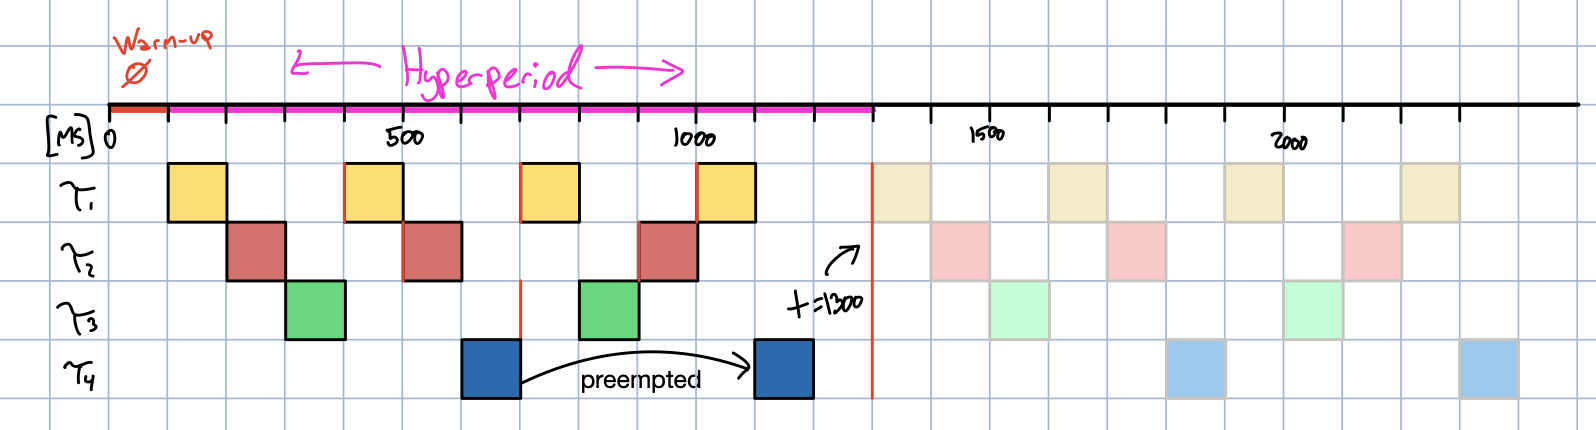
\includegraphics[width=\linewidth]{4-1-rms2-schedule}
\end{figure}
RMS2 output:
\begin{figure}[H]
        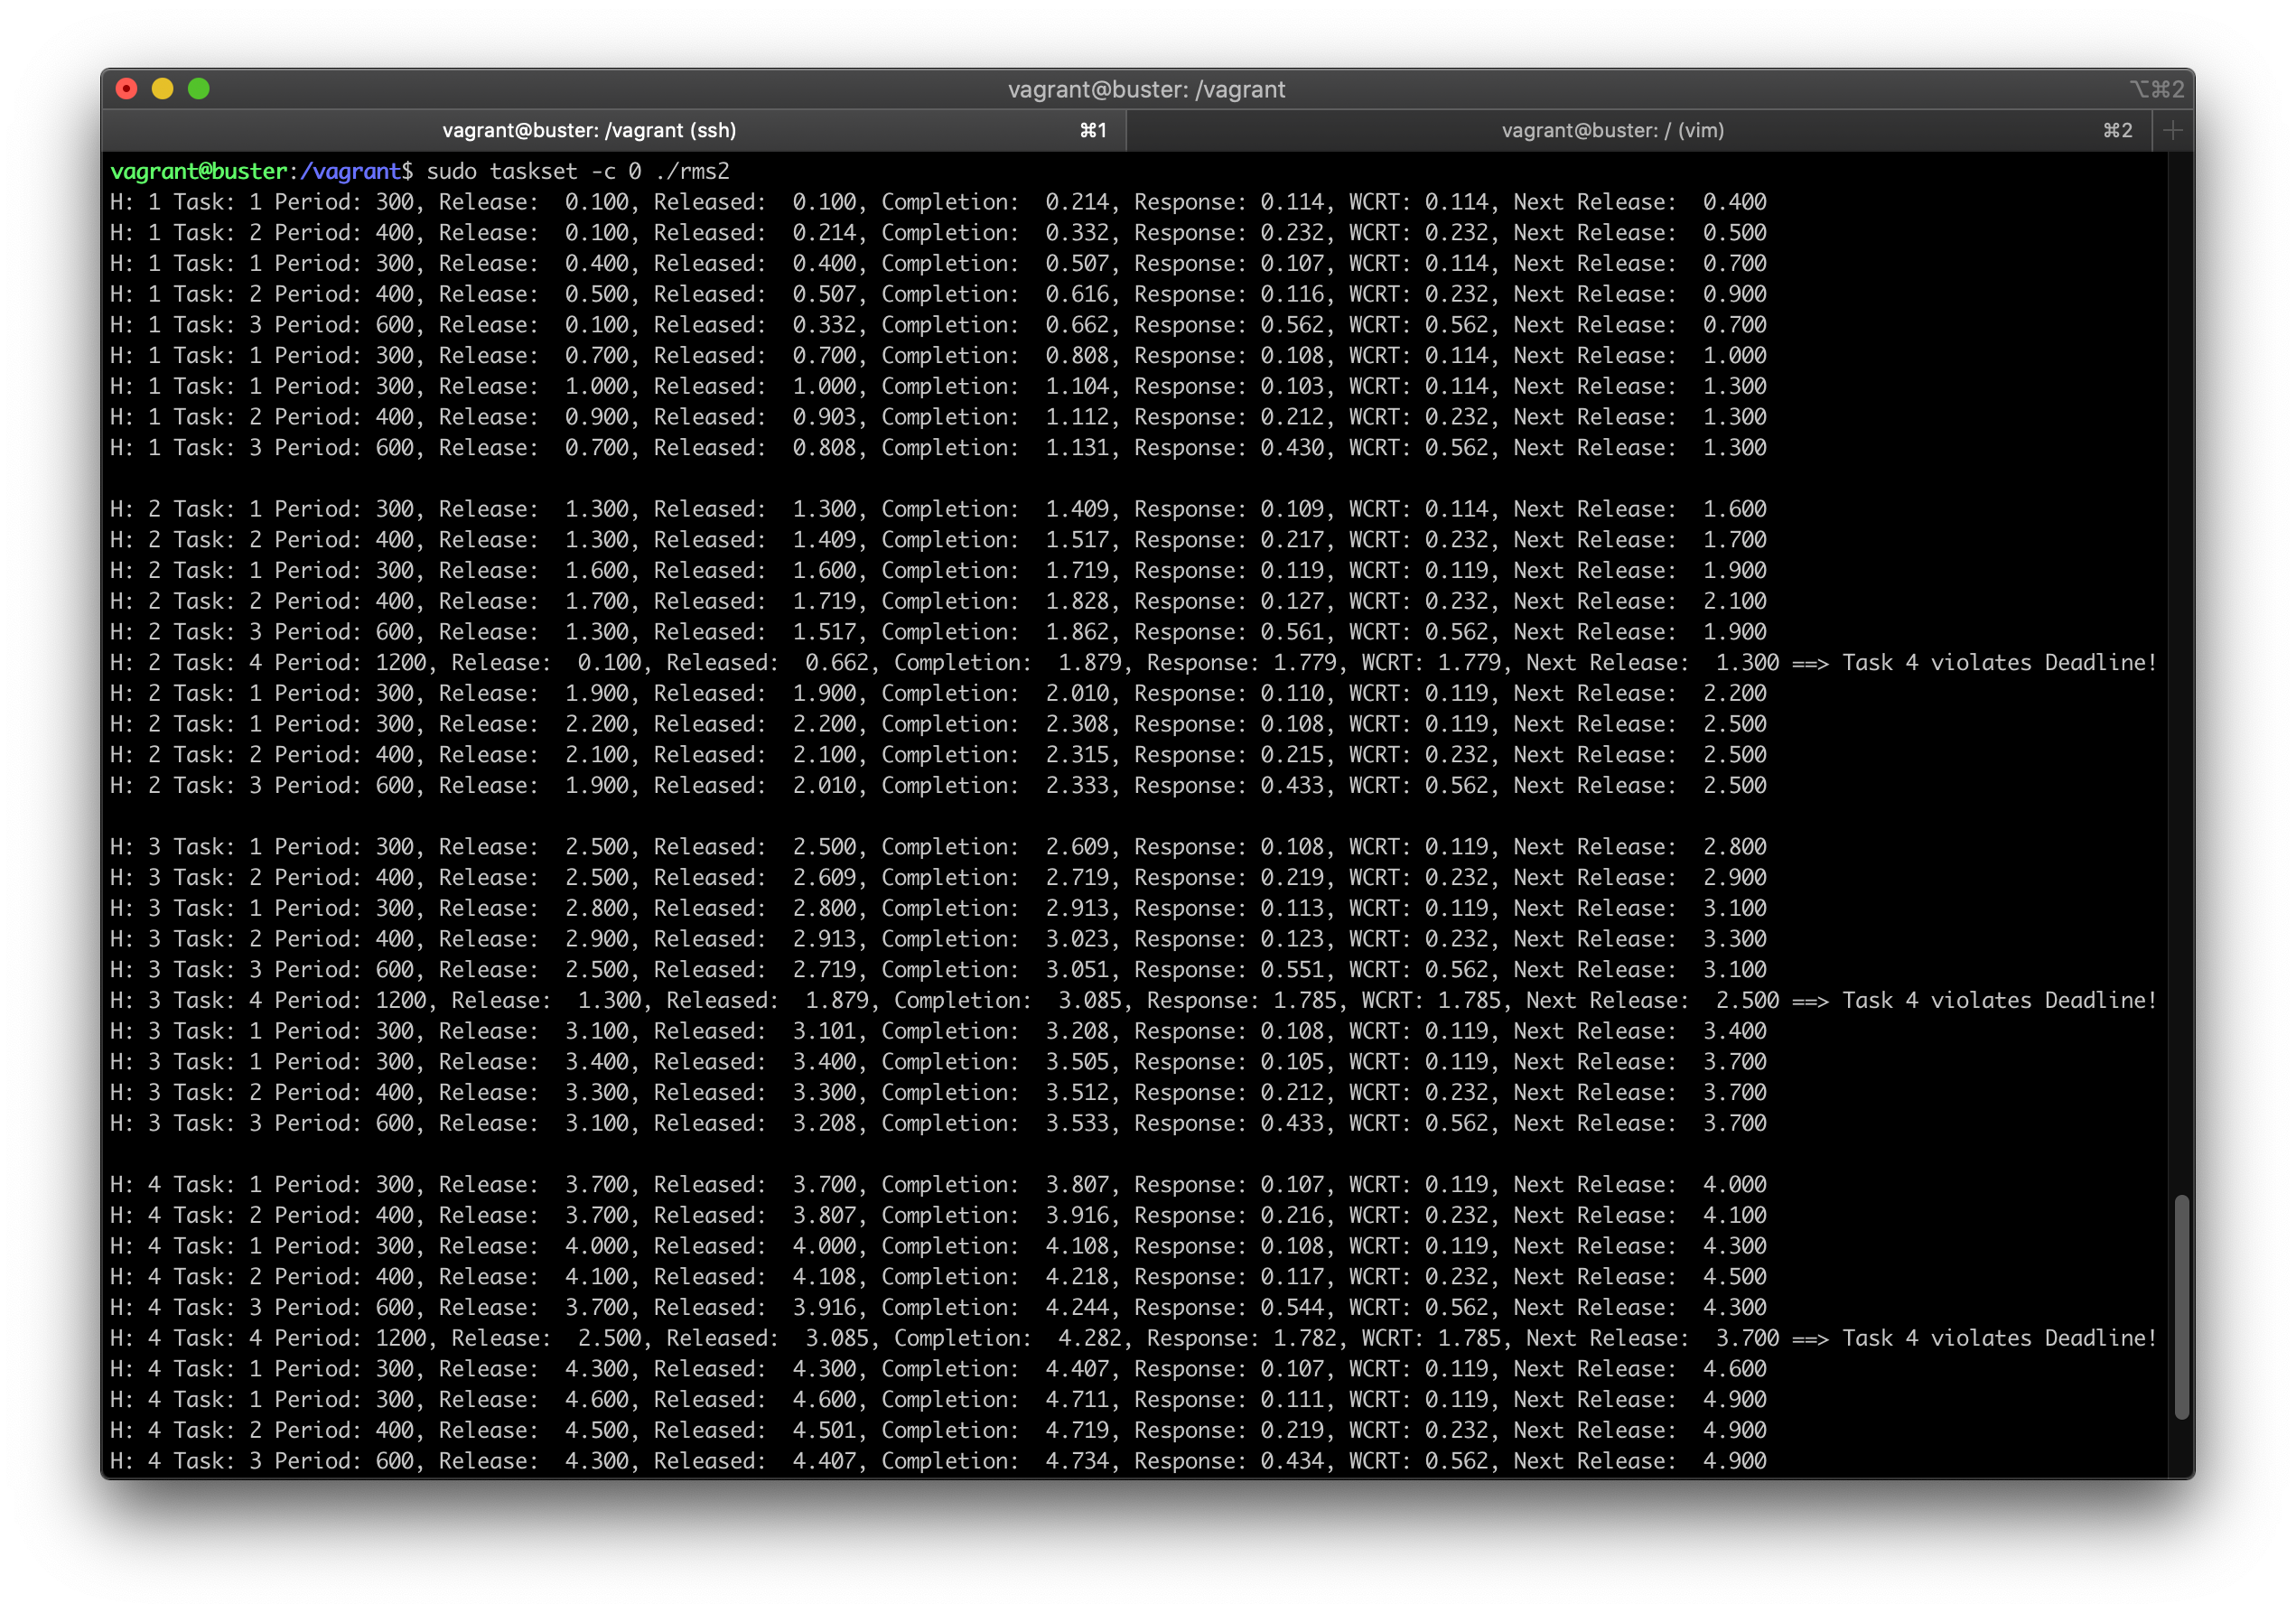
\includegraphics[width=\linewidth]{4-rms2-output}
\end{figure}
\end{enumerate}
